% % % % % % % % % % % % % % % % % % % % % %
% % % % % % Inicio del preámbulo % % % % % %
% % % % % % % % % % % % % % % % % % % % % %
\documentclass[12pt,a4paper]{report}

\usepackage[utf8]{inputenc}
\usepackage[spanish]{babel}
\usepackage{graphicx}

\usepackage[left=2cm,right=2cm,top=2cm,bottom=2cm,includeheadfoot]{geometry} % Para introducir texto en el margen
\usepackage{multicol}
\pagestyle{plain}

% % Configuración de márgenes
\setlength{\footskip}{2cm} % Distancia entre texto y final del pie

% % Configuración de tablas
\vspace{4cm} % Distancia vertical entre tablas
\renewcommand{\arraystretch}{1.3} % Espacio entre filas
% % % % % % % % % % % % % % % % % % % % % % % % % % % % % % %
% % % % % % Fin del preambulo e inicio del cuerpo % % % % % %
% % % % % % % % % % % % % % % % % % % % % % % % % % % % % % %

\begin{document}
% % Primera página del documento
\begin{titlepage}
    \begin{scriptsize}\noindent Facultad de Informática.\\
        Ingeniería en Informática.\\
        Ingeniería del Software.\\
        Proyecto: Everywhere House Control.
    \end{scriptsize}\\
    \vfill
    \begin{center}
        \begin{Large}
            \textbf{Proyecto IS}
        \end{Large}
    \end{center}
    \vfill
    \begin{flushright}
        \begin{scriptsize}
            \begin{tabular}{lll}
                Creado por & Gutierrez, Hector & Guzman, Fernando\\
                & Ladrón, Alejandro & Maldonado, Miguel Alexander\\
                & Morales, Álvaro & Ochoa, Victor\\
                & Rey, José Antonio & Saavendra, Luis Antonio\\
                & Tirado, Colin & Vicente, Victor\\
            \end{tabular}
        \end{scriptsize}
    \end{flushright}
\end{titlepage}
\thispagestyle{empty}
\cleardoublepage
\newpage

% % Tabla de contenidos, etc.
\pagenumbering{Roman}
\tableofcontents
\newpage
\thispagestyle{empty}
\cleardoublepage
\newpage
\pagenumbering{arabic}
\raggedbottom
\interfootnotelinepenalty 10000

% % % % % % % % % % % % % % % % % % % % % % % % % % % % % % %
% % % % % % % %  % Añadir archivos externos % % % % % % % % %
% % % % % % % % % % % % % % % % % % % % % % % % % % % % % % %

    \begin{tabular}{|p{3cm}|p{1.5cm}|p{3.5cm}|p{4cm}|}
    \hline
    \textbf{Fecha} & \textbf{Versión} & \textbf{Descripción} & \textbf{Autor} \\
    \hline
    26/11/2013 & 0.1 & Propuesta inicial & Maldonado, Miguel Alexander \\
    \hline
    04/12/2013 & 0.2 & Revisión & Tirado, Colin \\
    \hline
    10/12/2013 & 1.0 & Documento pasado a LaTeX & Tirado, Colin \\
    \hline
    15/12/2013 & 1.1 & Vision y ERS reestructurados & Ochoa, Víctor \\
    \hline
    17/12/2013 & 1.2 & - Reestructuracion de directorios\newline -Esquemas de todos los documentos a desarrollar incluidos & Ochoa, Víctor \\
    \hline
    04/01/2014 & 1.3 & Casos de uso incluidos & Tirado, Colin \\
    \hline
    10/01/2014 & 1.4 & Apartados de Introducci\'on, Representaci\'on del sistema y objetivos del documento de dise\~no & Tirado, Colin \\
    \hline
    11/01/2014 & 1.5 & Documento de gestión y planificación & Ladrón, Alejandro \\
    \hline
    16/01/2014 & 1.6 & Documento de dise\~no completado a falta de insertar im\'agenes. & Tirado, Colin \\
    \hline
    20/01/2014 & 1.7 & Documento ERS & Ochoa, Víctor \\
    \hline
    21/01/2014 & 1.8 & Imágenes de diseño insertadas & Tirado, Colin \\
    \hline
    21/01/2014 & 1.9 & Documento de gestión de Riesgos & Maldonado, Miguel Alexander\\
    \hline
    21/01/2014 & 1.10 & Documento de pruebas & Gutierrez, Hector \\
    \hline
    20/05/2014 & 1.11 & Revisión del documento de Visión & Tirado Colin \\
    \hline
\end{tabular}


    % % Primera página del documento
\begin{titlepage}
    \begin{scriptsize}\noindent Facultad de Informática.\\
        Ingeniería en Informática.\\
        Ingeniería del Software.\\
        Proyecto: Everywhere House Control.
    \end{scriptsize}\\
    \vfill
    \begin{center}
        \begin{Large}
            \textbf{Visión}
        \end{Large}
    \end{center}
    \vfill
    \begin{flushright}
        \begin{scriptsize}
            \begin{tabular}{lll}
                Creado por & Gutierrez, Hector & Guzman, Fernando\\
                & Ladrón, Alejandro & Maldonado, Miguel Alexander\\
                & Morales, Álvaro & Ochoa, Victor\\
                & Rey, José Antonio & Saavendra, Luis Antonio\\
                & Tirado, Colin & Vicente, Victor\\
            \end{tabular}
        \end{scriptsize}
    \end{flushright}
\end{titlepage}
\thispagestyle{empty}
\cleardoublepage
\newpage

% % Tabla de contenidos, etc.
\pagenumbering{Roman}
\tableofcontents
\newpage
\thispagestyle{empty}
\cleardoublepage
\newpage
\pagenumbering{arabic}
\raggedbottom
\interfootnotelinepenalty 10000

\chapter{Introducción}

\section{Propósito}
    El presente documento tiene como objetivo mostrar al lector el objetivo, requisitos y funcionalidades que ofrece el sistema \textit{Everywhere House Control} (EHC). \par
    Se recoge, analiza y define las necesidades de alto nivel y las características de un sistema que gestiona y automatiza los recursos del hogar (o centro de trabajo) a través de un dispositivo móvil de forma remota.

\section{Alcance}
    El sistema EHC será una aplicación ejecutable en cualquier dispositivo móvil que permitirá administrar y controlar los recursos del hogar (o centro de trabajo), ya sea tanto dentro como fuera del mismo.

\section{Definiciones, acrónimos y abreviaciones}
    \subsection{Del sistema}
        \begin{itemize}
            \item { \bf EHC}: Siglas correspondientes al nombre del sistema desarrollado (Everywhere House Control)
            \item { \bf Scrum}: Marco de trabajo para la gestión y desarrollo del software. Se trata de un proceso que se aplican de manera regular un conjunto de buenas prácticas para trabajar colaborativamente (en equipo). Se realizan entregas parciales y regulares del producto final, por lo que este tipo de proceso está especialmente recomendado para entornos complejos, donde se necesitan tener resultados pronto. \href{http://es.wikipedia.org/wiki/Scrum}{Scrum} se ejecuta en bloques temporales cortos y fijos (puede ser semanales, quincenales...), donde cada uno de ellos debe de producir un resultado que beneficiará al incremento del producto final. 
            \item { \bf Entorno EHC}: Hogar o lugar de trabajo donde se implanta el sistema.
        \end{itemize}
    \subsection{De tecnología}
    	\begin{itemize}
    		\item {\bf \href{http://es.wikipedia.org/wiki/Universal_Plug_and_Play}{PnP}}: es un conjunto de protocolos de comunicación que permite a periféricos en red, como ordenadores personales, impresoras, pasarelas de Internet, puntos de acceso Wi-Fi y dispositivos móviles, descubrir de manera transparente la presencia de otros dispositivos en la red y establecer servicios de red de comunicación, compartición de datos y entretenimiento.
    		\item {\bf X10 }: Es un protocolo de comunicaciones para el control remoto de dispositivos eléctricos, que utiliza la línea eléctrica (220V o 110V) preexistente, para transmitir señales de control entre equipos de automatización del hogar (domótica) en formato digital.
    		\item {\bf EIB}: (European Installation Bus) Es un sistema domótico que se desarrollo bajo el
    		amparo de la Unión Europea, con el objetivo de disminuir el número de importaciones de
    		productos del mismo tipo provenientes de los mercados japoneses y norteamericanos,
    		donde este tipo de tecnologías estaban más desarrolladas.
    		\item {\bf TCP/IP}: La familia de protocolos de Internet es un conjunto de protocolos de red en los que se basa Internet y que permiten la transmisión de datos entre computadoras. En ocasiones se le denomina conjunto de protocolos TCP/IP, en referencia a los dos protocolos más importantes que la componen: Protocolo de Control de Transmisión (TCP) y Protocolo de Internet (IP), que fueron dos de los primeros en definirse, y que son los más utilizados de la familia. 
    	\end{itemize}
    	

\section{Referencias}
    \begin{itemize}
        \item Glosario
        \item Plan de desarrollo software
        \item Scrum
        \item Diagrama de casos de uso
        \item Guías de estilo
    \end{itemize}

\chapter{Posicionamiento}

\section{Perspectivas del producto}
    El sistema EHC será un producto dise\~nado para la administración y el control de los recursos del hogar (o centro de trabajo), ya sea tanto dentro como fuera del mismo. Además permitirá que dichas tareas (administración y control) se hagan de una manera centralizada a trav\'es de un único dispositivo.

    EHC se servirá de un servidor y una base de datos para la gestión y administración de perfiles de usuario así como la conexión de los mismos al sistema. La conexión de los usuarios al sistema EHC podrá establecerse tanto dentro como fuera del lugar en el que est\'e implantado el sistema.

    El producto tendrá una aplicación ejecutable en cualquier dispositivo móvil, así como su correspondiente versión web y PC. Dicha aplicación se compondrá de interfaces gráficas intuitivas, sencillas y amigables para cualquier tipo de usuario.

\section{Oportunidad de negocio}
    Este sistema permitirá al usuario tener un control absoluto en el entorno EHC sobre los recursos del mismo (tales como; activar calefacción, subir/bajar persianas, grabar programas de televisión, apagar/encender luces, apagar/encender enchufes, etc.), pudiendo acceder de manera fácil y rápida a cualquier recurso gracias a interfaces gráficas sencillas y amigables.

\section{Sentencia que define el problema}
    \begin{tabular}{|p{6cm}|p{10cm}|}
        \hline \textbf{El problema de} & Controlar y gestionar una serie de recursos un lugar determinado.\\
        \hline \textbf{Afecta a} & Toda persona/empresa que necesite controlar o gestionar un lugar determinado de forma remota.\\
        \hline \textbf{El impacto asociado es} & Controlar desde uno o varios dispositivos aquellos elementos del entorno EHC \\
        \hline \textbf{Una solución adecuada sería} & Automatizar ciertos elementos críticos para el usuario/empresa del entorno EHC para que después sean controlados a través de una aplicación móvil o web desde cualquier lugar. \par
        Este control sobre el entorno EHC puede ser de forma directa a través de Internet o a través de ordenes planificadas gestionadas anteriormente por el usuario.\\
        \hline
    \end{tabular}

\section{Sentencia que define la posición del producto}
    \begin{tabular}{|p{6cm}|p{10cm}|}
        \hline \textbf{Para} &  Usuario (o empresa) que desee  tener de manera centralizada el control de los recursos del entorno EHC.\\
        \hline \textbf{Quienes} & Necesiten controlar de forma remota un entorno EHC.\\
        \hline \textbf{El nombre del producto} & Es un sistema hardware y software de control y gestión de elementos de forma remota. \\
        \hline \textbf{Que} & Proporciona un entorno más agradable al usuario en el hogar, y por lo tanto, afecta a la calidad de vida del usuario.\\
        \hline \textbf{No como} & Las aplicaciones actuales de domotización de hogares donde solo se hacen cargo de realizar peticiones a elementos de casa y con un elevado coste de hardware e instalación. \\
        \hline \textbf{Producto} & Permite gestionar los distintos recursos que ofrezca el lugar donde se encuentre implantado el sistema EHC mediante una interfaz gráfica sencilla y amigable. Además proporciona un acceso rápido y eficiente al sistema desde cualquier punto con acceso a Internet o a través de tareas programadas. \par
        La instalación del sistema en un posible futuro entorno EHC se realiza a un bajo coste y sin necesidad de alterar la estructura del hogar. \\
        \hline
    \end{tabular}

\section{Futuro mercado del sistema}
    La domótica es una herramienta que está creciendo en nuestro país en los últimos años, pero a día de hoy, no está tan extendido como podría estarlo debido a su alto coste tanto económico como de instalación. Los sistemas actuales de domótica necesitan una gran instalación ya que abarcan todos los elementos del hogar y los usuarios se muestran reacios a realizar una obra para domotizar el hogar, por lo que la gran mayoría que dispone de esta herramienta han adquirido el hogar domotizado.
    \par
    El sistema EHC se centra en el usuario que no desee realizar una instalación domótica que implique alterar/modificar la estructura del hogar y a un alto coste económico, por lo que el sistema se mueve en un mercado muy amplio ya que es la manera más fácil de domotizar un hogar.
    \par
    Se ofrece una instalación más cómoda y personalizada con este sistema, ya que   debido a la fácil instalación del sistema los usuarios no se muestran reacios a domotizar el hogar y pueden probar gradualmente a instalar nuestro sistema en el entorno EHC sin necesidad de hacer modificaciones en un lugar concreto.
    \par
    Al contrario que toda empresa de domótica, donde el modelo de negocio de esta empresa se centra en la instalación y mantenimiento de los componentes instalados, el sistema EHC se centra en una instalación a bajo coste y a una suscripción mensual con distintas con distintos perfiles según la suscripción seleccionada por el usuario.

\chapter{Descripción de Stakeholders y usuarios}
    Para proveer de una forma efectiva el servicio y que se ajuste a las necesidades de los usuarios, es necesario identificar e involucrar a todos los participantes en el proyecto como parte del proceso de modelado de requerimientos. También es necesario identificar a los usuarios del sistema y asegurarse de que el conjunto de participantes en el proyecto los representa adecuadamente. Esta sección muestra un perfil de los participantes y de los usuarios involucrados en el proyecto, así como los problemas más importantes que éstos perciben para enfocar la solución propuesta hacia ellos. No describe sus requisitos específicos pero proporciona la justificación de por qué estos requisitos son necesarios.

\section{Resumen de \textit{Stakeholders}}
    \begin{tabular}{|p{4cm}|p{3cm}|p{10cm}|}
        \hline \textbf{Nombre} &  \textbf{Descripción} & \textbf{Responsbilidades} \\
        \hline Morales Lozano, Álvaro & Representante Global de la empresa EHC. &
        \begin{itemize}
            \item Seguimiento del desarrollo del proyecto a nivel global.
            \item Aprueba requisitos y funcionalidades a nivel global.
        \end{itemize} \\
        \hline Vicente Sánchez, Victor & Representante del Departamento de Software. &
        \begin{itemize}
            \item Seguimiento del desarrollo del proyecto a nivel software.
            \item Aprueba requisitos y funcionalidades.
        \end{itemize} \\
        \hline Gutiérrez, Héctor & Representante del Departamento de Hardware. &
        \begin{itemize}
            \item Seguimiento del desarrollo del proyecto a nivel hardware.
            \item Aprueba requisitos y funcionalidades.
        \end{itemize} \\
        \hline Ladrón De Guevara, Alejandro & Representante del Departamento de Servidor.&
        \begin{itemize}
            \item Seguimiento del desarrollo del proyecto a nivel servidor.
            \item Aprueba requisitos y funcionalidades.
        \end{itemize} \\
        \hline
    \end{tabular}

\section{Resumen de usuarios}
    \begin{tabular}{|p{3cm}|p{7cm}|p{6cm}|}
        \hline \textbf{Nombre} &  \textbf{Descripción} & \textbf{StakeHolder} \\
        \hline Administrador & Encargado de la instalación del sistema EHC en el cliente. Se encargará de  instalar/configurar el sistema en el entorno EHC. & Gutiérrez, Hector \\
        \hline Usuario & Participante del entorno EHC &   Ladrón De Guevara, Alejandro \par Vicente Sánchez, Victor \\
        \hline
    \end{tabular}

\section{Entorno de usuarios}
    Los usuarios entrarán al sistema identificándose sobre cualquier dispositivo móvil que tenga instalada la aplicación de gestión del sistema EHC o a través de la aplicación web. Tras este paso podrán controlar multitud de tareas y acciones que ofrecen los distintos recursos del entorno EHC navegando a través de interfaces ágiles y amigables.

\section{Perfil de \textit{Stakeholders}}
    \subsection{Departamento de Software}
        \begin{tabular}{|p{4cm}|p{12cm}|}
            \hline \textbf{Representante} & Vicente Sánchez, Victor. \\
            \hline \textbf{Descripción} & Representante del Departamento de Software. \\
            \hline \textbf{Tipo} &  [Experto] Estudiante de sistemas software. \\
            \hline \textbf{Responsabilidades} &  Llevar a cabo un seguimiento del desarrollo del proyecto y aprobación de  los requisitos y funcionalidades del sistema a nivel software.\\
            \hline \textbf{Criterio de éxito} &  [A definir por el cliente]\\
            \hline \textbf{Grado de participación} &  Revisión de requerimientos, desarrollo y estructura del sistema a nivel software.\\
            \hline \textbf{Comentarios} &  Ninguno\\
            \hline
        \end{tabular}

        \begin{tabular}{|p{4cm}|p{12cm}|}
            \hline \textbf{Representante} &  Maldonado Lenis, Miguel Alexander. \\
            \hline \textbf{Descripción} &  Componente del Departamento de Software.\\
            \hline \textbf{Tipo} &  [Experto] Estudiante de sistemas software.\\
            \hline \textbf{Responsabilidades} &  Desarrollar requisitos y funcionalidades del sistema a nivel software.\\
            \hline \textbf{Criterio de éxito} & [A definir por el cliente]\\
            \hline \textbf{Grado de participación} & Funcional. Llevando a cabo en los plazos planificados las tareas que le van siendo asignadas por el coordinador.\\
            \hline \textbf{Comentarios} &  Ninguno.\\
            \hline
        \end{tabular}
        
		\begin{tabular}{|p{4cm}|p{12cm}|}
            \hline \textbf{Representante} & Tirado, Colin \\
            \hline \textbf{Descripción} & Componente del Departamento de Software. \\
            \hline \textbf{Tipo} & [Experto] Estudiante de sistemasde gestión. \\
            \hline \textbf{Responsabilidades} & Llevar a cabo un seguimiento del desarrollo del proyecto con la finalidad de recopilar información para elaborar y mantener la documentación del mismo. Y desarrollar requisitos y funcionalidades del sistema a nivel software. \\
            \hline \textbf{Criterio de éxito} & [A definir por el cliente] \\
            \hline \textbf{Grado de participación} & Revisión, elaboración y mantenimiento de la documentación. Y realización en los plazos planificados de las tareas que le van siendo asignadas por el coordinador.  \\
            \hline \textbf{Comentarios} &  Ninguno. \\
            \hline
        \end{tabular}

    \subsection{Departamento de Hardware}

        \begin{tabular}{|p{4cm}|p{12cm}|}
            \hline \textbf{Representante} & Morales Lozano, Álvaro \\
            \hline \textbf{Descripción} &  Componente del Departamento de Hardware. Y representante global de la empresa EHC. \\
            \hline \textbf{Tipo} &  [Experto] Estudiante de gestión de sistemas.\\
            \hline \textbf{Responsabilidades} &  Encargado de mostrar las necesidades de cada usuario del sistema. Además, llevar a cabo un seguimiento del desarrollo del proyecto y aprobación de  los requisitos y funcionalidades del sistema a nivel global y a nivel hardware.\\
            \hline \textbf{Criterio de éxito} &  [A definir por el cliente]\\
            \hline \textbf{Grado de participación} &  Revisión de requerimientos, desarrollo y estructura del sistema a nivel global. Y realización en los plazos planificados de las tareas que le van siendo asignadas por el coordinador.\\
            \hline \textbf{Comentarios} &  Ninguno.\\
            \hline
        \end{tabular}

        \begin{tabular}{|p{4cm}|p{12cm}|}
            \hline \textbf{Representante} &  Gutiérrez, Héctor\\
            \hline \textbf{Descripción} &  Representante del Departamento de Hardware. \\
            \hline \textbf{Tipo} &  [Experto] Estudiante de sistemas hardware.\\
            \hline \textbf{Responsabilidades} &  Llevar a cabo un seguimiento del desarrollo del proyecto y aprobación de  los requisitos y funcionalidades del sistema a nivel hardware. \\
            \hline \textbf{Criterio de éxito} &  [A definir por el cliente]\\
            \hline \textbf{Grado de participación} &  Revisión de requerimientos, desarrollo y estructura del sistema a nivel hardware.\\
            \hline \textbf{Comentarios} &  Ninguno\\
            \hline
        \end{tabular}
        
        \begin{tabular}{|p{4cm}|p{12cm}|}
            \hline \textbf{Representante} & Guzman, Fernando \\
            \hline \textbf{Descripción} & Componente del Departamento de Hardware. \\
            \hline \textbf{Tipo} & [Experto] Estudiante de sistemas hardware. \\
            \hline \textbf{Responsabilidades} & Desarrollar requisitos y funcionalidades del sistema a nivel hardware. \\
            \hline \textbf{Criterio de éxito} & [A definir por el cliente] \\
            \hline \textbf{Grado de participación} & Funcional. Llevando a cabo en los plazos planificados las tareas que le van siendo asignadas por el coordinador. \\
            \hline \textbf{Comentarios} &  Ninguno \\
            \hline
        \end{tabular}
        
		\begin{tabular}{|p{4cm}|p{12cm}|}
            \hline \textbf{Representante} & Ochoa, Victor \\
            \hline \textbf{Descripción} & Componente del Departamento de Hardware. \\
            \hline \textbf{Tipo} & [Experto] Estudiante de sistemas de gestión. \\
            \hline \textbf{Responsabilidades} & Llevar a cabo un seguimiento del desarrollo del proyecto con la finalidad de recopilar información para elaborar y mantener la documentación del mismo. Y desarrollar requisitos y funcionalidades del sistema a nivel hardware. \\
            \hline \textbf{Criterio de éxito} & [A definir por el cliente] \\
            \hline \textbf{Grado de participación} & Revisión, elaboración y mantenimiento de la documentación. Y realización en los plazos planificados de las tareas que le van siendo asignadas por el coordinador. \\
            \hline \textbf{Comentarios} &  Ninguno. \\
            \hline
        \end{tabular}

    \subsection{Departamento de Servidor}
        \begin{tabular}{|p{4cm}|p{12cm}|}
            \hline \textbf{Representante} &  Ladrón De Guevara, Alejandro\\
            \hline \textbf{Descripción} & Representante del Departamento de Servidor. \\
            \hline \textbf{Tipo} &  [Experto] Estudiante de sistemas con servidores. \\
            \hline \textbf{Responsabilidades} & Llevar a cabo un seguimiento del desarrollo del proyecto y aprobación de  los requisitos y funcionalidades del sistema a nivel del servidor. \\
            \hline \textbf{Criterio de éxito} & [A definir por el cliente] \\
            \hline \textbf{Grado de participación} & Revisión de requerimientos, desarrollo y estructura del sistema a nivel del servidor. \\
            \hline \textbf{Comentarios} &  Ninguno. \\
            \hline
        \end{tabular}

        \begin{tabular}{|p{4cm}|p{12cm}|}
            \hline \textbf{Representante} & Rey, José Antonio \\
            \hline \textbf{Descripción} & Componente del Departamento de Servidor  \\
            \hline \textbf{Tipo} & [Experto] Estudiante de sistemas con servidores. \\
            \hline \textbf{Responsabilidades} & Desarrollar requisitos y funcionalidades del sistema a nivel del servidor. \\
            \hline \textbf{Criterio de éxito} & [A definir por el cliente] \\
            \hline \textbf{Grado de participación} & Funcional. Llevando a cabo en los plazos planificados las tareas que le van siendo asignadas por el coordinador. \\
            \hline \textbf{Comentarios} & Ninguno. \\
            \hline
        \end{tabular}

        \begin{tabular}{|p{4cm}|p{12cm}|}
            \hline \textbf{Representante} & Saavedra, Luis Antonio \\
            \hline \textbf{Descripción} & Componente del Departamento de Servidor \\
            \hline \textbf{Tipo} & [Experto] Estudiante de sistemas con servidores. \\
            \hline \textbf{Responsabilidades} & Desarrollar requisitos y funcionalidades del sistema a nivel del servidor. \\
            \hline \textbf{Criterio de éxito} & [A definir por el cliente] \\
            \hline \textbf{Grado de participación} & Funcional. Llevando a cabo en los plazos planificados las tareas que le van siendo asignadas por el coordinador. \\
            \hline \textbf{Comentarios} & Ninguno. \\
            \hline
        \end{tabular}

\section{Tipos de usuario}

    \subsection{Administrador}
        \begin{tabular}{|p{4cm}|p{12cm}|}
            \hline \textbf{Representante} & Administrador \\
            \hline \textbf{Descripción} & Participante directo de la empresa EHC que se encarga de la instalación y el aprendizaje inicial del sistema EHC en el entorno instalado. \\
            \hline \textbf{Tipo} & Usuario casual del sistema. \\
            \hline \textbf{Responsabilidades} & Responsable de la instalación y del funcionamiento del sistema. \\
            \hline \textbf{Criterio de éxito} & [A definir por el cliente] \\
            \hline \textbf{Grado de participación} & Instalación del sistema en el lugar contratado. \par
            Mostrar y aconsejar al usuario como usar el sistema. \\
            \hline \textbf{Comentarios} & Ninguno. \\
            \hline
        \end{tabular}

    \subsection{Cliente}
        \begin{tabular}{|p{4cm}|p{12cm}|}
            \hline \textbf{Representante} & Cliente. \\
            \hline \textbf{Descripción} & Usuario (o empresa) que desee  tener de manera centralizada el control de los recursos del hogar (o centro de trabajo). \\
            \hline \textbf{Tipo} & Usuario casual del sistema. \\
            \hline \textbf{Responsabilidades} & Uso correcto de la instalación del sistema EHC \\
            \hline \textbf{Criterio de éxito} & [A definir por el cliente] \\
            \hline \textbf{Grado de participación} & [A definir por el cliente] \\
            \hline \textbf{Comentarios} & Ninguno. \\
            \hline
        \end{tabular}

\section{Alternativas y competencias}
    A continuación, se mostrará una lista de las principales alternativas al sistema:\\
    \begin{itemize}
    \item {\bf OpenDomotica} -  https://opendomotica.wordpress.com/
            \begin{tabbing}
            ---- \= ------ \= ----- \= ----- \...\kill
            \>\> {\bf Autor/es}: Juan Antonio Infantes Díaz (Dirigido por David Santo Orcero)\\
            \>\> {\bf Inicio}: Noviembre del 2008.\\
            \>\> {\bf Objetivo}: Entorno domótico libre.\\
            \>\> {\bf Tecnologias utilizadas}:\\
            \>\>\> {\bf Arduino}: Hardware libre.\\
            \>\>\> {\bf Mister House}: Software libre.\\
            \end{tabbing}
               
     \item {\bf OpenDomo} - http://es.opendomo.org/
     		\begin{tabbing}
     		---- \= ------ \= ----- \= ----- \...\kill
            \>\> {\bf Autor/es}: Daniel Lerch y Oriol Palenzuela.\\
            \>\> {\bf Inicio}: 2006.\\
            \>\> {\bf Objetivo}: Ofrece servicios básicos de todo sistema de control domótico.\\
            \>\> {\bf Origen}: Surgió de la necesidad de unificar las diferentes tecnologías domóticas\\\>\>\> como: uPnP, X10, EIB, etc, con el protocolo TCP/IP.\\
            \>\> {\bf Comentarios}: Han desarrollado una software domotico bajo Arduino llamado\\\>\>\> "Domino".\\
            \end{tabbing}
    \end{itemize}
    
\chapter{Descripci�n global del producto}

\section{Perspectiva del producto}
    El producto a desarrollar es un sistema que gestiona y automatiza los recursos de un entorno EHC a trav�s de un dispositivo m�vil de forma remota.

\section{Resumen de caracter�sticas}
    A continuaci�n se mostrar� un listado de beneficios que obtendr� el cliente a partir del producto: \\ \par
    \begin{tabular}{|p{8cm}|p{8cm}|}
        \hline \textbf{Beneficio del cliente} & \textbf{Caracter�sticas que lo apoyan} \\
        \hline & \\
        \hline
    \end{tabular}

\section{Suposiciones y dependencias}
    A continuaci�n se muestra una lista de suposiciones y dependencias del sistema que afectan al sistema y al cumplimiento de de lo especificado en los documentos del proyecto: \\ \par
    \begin{tabular}{|p{4cm}|p{6cm}|p{6cm}|}
        \hline \textbf{Categor�a} &  \textbf{Comentario} & \textbf{Limitaci�n si no se cumple} \\
        \hline Suposici�n & El usuario tiene en el hogar conexi�n a Internet & El usuario solo podr� usar el sistema  EHC de forma local. \\
        \hline Dependencia & El hogar dispone de forma ininterrumpida corriente el�ctrica & El sistema EHC no estar� disponible en esos periodos sin corriente el�ctrica \\
        \hline & & \\
        \hline
    \end{tabular}

\section{Costo y precio}
    TBD

\section{Licencia e instalaci�n}
    La instalaci�n y configuraci�n inicial ser� realizada por el personal de la empresa. Dicha instalaci�n y configuraci�n no solo se centra en el montaje de los elementos hardware necesarios para el funcionamiento del sistema, sino tambi�n en la configuraci�n de la red de comunicaci�n entre los distintos dispositivos que se encuentran en el entorno EHC. \par

    Tras dicha instalaci�n, se entregar� al usuario una licencia de uso del sistema EHC con sus correspondientes claves de identificaci�n y uso del sistema.

\chapter{Funcionalidades del sistema [Son los requisitos de Usuario]}

\section{Control remoto del sistema}
	El sistema garantiza el control y gesti�n de los distintos dispositivos instalados en el espacio EHC tanto de forma local como a trav�s de Internet.

\section{Creaci�n de perfiles}
	La uso de m�ltiplos perfiles de mandatos facilita el control de los dispositivos del espacio EHC. Es posible crear perfiles adaptados a los usuarios del hogar como por ejemplo  a ni�os, vecinos, padres...

\section{Sistemas de alarmas}
	No solo se centra el sistema en la gesti�n y control del espacio EHC, sino que tambi�n ofrece herramientas de seguridad como:
	\begin{itemize}
		\item Videoc�mara: el usuario podr� ver en tiempo real un espacio determinado donde est� localizado una c�mara. s
		\item Sensor meteorol�gico: el usuario podr� ser notificado de un estado concreto del tiempo del espacio EHC
	\end{itemize}

\section{Seguridad de la aplicaci�n}
	TBD (<seguridad app, conexi�n local, conexi�n arduino-aparato>)

\section{Programas de eventos}
	Es posible programa eventos del espacio EHC para que se inicien en un momento determinado. Esto facilita la gesti�n del usuario sobre el espacio EHC para realizar operaciones peri�dicas durante temporadas de vacaciones o por otros motivos.

\chapter{Documentación}

\section{Manual de usuario}

\section{Ayuda en línea}

\section{Guías de instalación, configuración y fichero léame}

\section{Página web}

\section{Wiki}


% % % % % % Fin del cuerpo

    % % Primera página del documento
\begin{titlepage}
    \begin{scriptsize}\noindent Facultad de Informática.\\
        Ingeniería en Informática.\\
        Ingeniería del Software.\\
        Proyecto: Everywhere House Control.
    \end{scriptsize}\\
    \vfill
    \begin{center}
        \begin{Large}
            \textbf{Gestion y planificacion}
        \end{Large}
    \end{center}
    \vfill
    \begin{flushright}
        \begin{scriptsize}
            \begin{tabular}{lll}
                Creado por & Gutierrez, Hector & Guzman, Fernando\\
                & Ladrón, Alejandro & Maldonado, Miguel Alexander\\
                & Morales, Álvaro & Ochoa, Victor\\
                & Rey, José Antonio & Saavendra, Luis Antonio\\
                & Tirado, Colin & Vicente, Victor\\
            \end{tabular}
        \end{scriptsize}
    \end{flushright}
\end{titlepage}
\thispagestyle{empty}
\cleardoublepage
\newpage

% % Tabla de contenidos, etc.
\pagenumbering{Roman}
\tableofcontents
\newpage
\thispagestyle{empty}
\cleardoublepage
\newpage
\pagenumbering{arabic}
\raggedbottom
\interfootnotelinepenalty 10000

%\input{2.Gestion&Planificacion...}
%\chapter{Introducci�n}

    ***********************\newline
    TODO: Las secciones que estan recogidas en esta Introduccion son requisitos que hay que clasificar convenientemente en los siguientes capitulos (los que distuinguen los tipos de requisitos)
    ***********************\newline

\section{Caracter�sticas del usuario}
    Los usuarios de la aplicaci�n deber�n estar registrados para poder acceder a ella. El sistema contar� con una base de datos donde estar�n almacenados los nombres de usuario y contrase\~nas. Dichos usuarios podr�n acceder a la aplicaci�n y hacer uso de ella.

    \subsection{Perfil del usuario}
        Cada usuario tendr� un perfil espec�fico para que su interacci�n con el sistema sea correcto y no conlleve a fallos:
        \begin{description}
            \item[Administrador del sistema] Usuario con gran conocimiento en el manejo del sistema con una previa capacitaci�n por parte de la empresa. Encargado de manejar el sistema con gran responsabilidad sobre los criterios de permisos de los usuarios.

            \item[Usuario principal] Persona que interactuar� continuamente con el sistema, su control sobre el mismo ha de ser eficiente. El conocimiento del manejo del sistema ser� adquirido por el usuario gracias a una peque\~na sesi�n de contacto guiada por el administrador, aunque la propia aplicaci�n estar� capacitada con una presentaci�n/tutorial guiada/o del uso de la misma.

            \item[Visitante] Persona que interactuar� ocasionalmente con el sistema, su control sobre el mismo ha de ser configurada por el usuario principal. El conocimiento del manejo del sistema ser� adquirido gracias a la presentaci�n/tutorial guiada/o del uso de la aplicaci�n.
        \end{description}

    \subsection{Jerarqu�a de usuarios}

\section{Restricciones}
    A continuaci�n se presenta una lista de restricciones impuestas por los desarrolladores del sistema:

    \subsection{Limitaciones de usuario}
        \begin{description}
            \item[Administrador] Ninguna limitaci�n.

            \item[Usuario principal] Tendr� la capacidad de crear perfiles de 'invitados' y configurar sus permisos, limitando as� posibles accesos no deseados. Se ver� mermado su control a la hora de a\~nadir y configurar m�s recursos al sistema.

            \item[Perfil de invitado] Su acceso a ciertas caracter�sticas del sistema se ver� limitado debido a las posibles restricciones de su perfil.
        \end{description}

    \subsection{Pol�ticas reguladoras}
        La aplicaci�n se desarrollar� mediante software de licencia abierta, por lo tanto no se deber� pagar por su uso. Asimismo, la utilizaci�n de la aplicaci�n se har� mediante las pol�ticas establecidas por este tipo de licenciamiento.

    \subsection{Limitaciones hardware}
        Para el completo funcionamiento de esta aplicaci�n ser� necesario un servidor y una serie de mecanismos hardware que se instalar�n en el lugar donde se quiera implantar el sistema EHC.

    \subsection{Interfaces con otras aplicaciones}
        Debido a que el sistema no interact�a con otros sistemas y es aut�nomo, no se desarrollar�n interfaces con otras aplicaciones. Las conexiones necesarias para la utilizaci�n del servidor y los mecanismos hardware, se har�n por medio de la configuraci�n de los mismos.


    \subsection{Funciones de control}
        El sistema EHC administrar� y controlar� los permisos que tiene cada usuario para que su accesibilidad se haga de una manera correcta, de tal forma que acceda a la informaci�n que le corresponde de acuerdo a sus permisos. Tambi�n deber� tener controles adecuados para la gesti�n y validaci�n de datos, as� como para las tareas, mandatos e instrucciones pedidos al sistema.

        Por otro lado, a cargo de varios supervisores estar�n encargadas las tareas de revisi�n de elementos como el c\'digo, el repositorio, fechas de entrega, documentaci�n, etc.

    \subsection{Requisitos del lenguaje}
        Tanto el material que vaya dirigido al usuario como la aplicaci�n deben estar en espa\~nol.

    \subsection{Lenguajes de programaci�n}
        Se har� uso de las tecnolog�as; Java (Android) y Objective-c (iOS).

    \subsection{Requisitos de fiabilidad}
        Previamente, para evitar posibles futuros fallos, la aplicaci�n ser� sometida a multitud de pruebas y tests garantizando que se entregar� al usuario un programa totalmente funcional y eficiente.

    \subsection{Suposiciones y dependencias}
        Se han supuesto los requisitos para que el sistema funcione correctamente con especificaciones est�ndar.
        Es viable tratar de ampliar la capacidad de mercado capacitando al sistema con versiones de la aplicaci�n en diferentes idiomas.

    \subsection{Requisitos futuros}
        En un futuro se tratar�n de implementar nuevas funcionalidades que requerir�n una modificaci�n de los requisitos iniciales:


% % % % % % Fin del cuerpo
    % % Primera página del documento
\begin{titlepage}
    \begin{scriptsize}\noindent Facultad de Informática.\\
        Ingeniería en Informática.\\
        Ingeniería del Software.\\
        Proyecto: Everywhere House Control.
    \end{scriptsize}\\
    \vfill
    \begin{center}
        \begin{Large}
            \textbf{Documento de análisis}
        \end{Large}
    \end{center}
    \vfill
    \begin{flushright}
        \begin{scriptsize}
            \begin{tabular}{lll}
                Creado por & Gutierrez, Hector & Guzman, Fernando\\
                & Ladrón, Alejandro & Maldonado, Miguel Alexander\\
                & Morales, Álvaro & Ochoa, Victor\\
                & Rey, José Antonio & Saavendra, Luis Antonio\\
                & Tirado, Colin & Vicente, Victor\\
            \end{tabular}
        \end{scriptsize}
    \end{flushright}
\end{titlepage}
\thispagestyle{empty}
\cleardoublepage
\newpage

% % Tabla de contenidos, etc.
\pagenumbering{Roman}
\tableofcontents
\newpage
\thispagestyle{empty}
\cleardoublepage
\newpage
\pagenumbering{arabic}
\raggedbottom
\interfootnotelinepenalty 10000

% % Primera p�gina del documento
\begin{titlepage}
    \begin{scriptsize}\noindent Facultad de Inform�tica.\\
        Ingenier�a en Inform�tica.\\
        Ingenier�a del Software.\\
        Proyecto: Everywhere House Control.
    \end{scriptsize}\\
    \vfill
    \begin{center}
        \begin{Large}
            \textbf{Especificaci�n de Requisitos de Software}
        \end{Large}
    \end{center}
    \vfill
    \begin{flushright}
        \begin{scriptsize}
            \begin{tabular}{lll}
            Creado por & Gutierrez, Hector & Guzman, Fernando  \\
                 & Ladr�n, Alejandro & Maldonado, Miguel Alexander \\
                 & Morales, �lvaro & Ochoa, Victor \\
                 & Rey, Jos� Antonio & Saavendra, Luis Antonio  \\
                 & Tirado, Colin & Vicente, Victor \\
            \end{tabular}
        \end{scriptsize}
    \end{flushright}
\end{titlepage}
\thispagestyle{empty}
\cleardoublepage
\newpage

% % Tabla de contenidos, etc.
\pagenumbering{Roman}
\tableofcontents
\newpage
\thispagestyle{empty}
\cleardoublepage
\newpage
\pagenumbering{arabic}
\raggedbottom
\interfootnotelinepenalty 10000

\chapter{Introducci�n}

    ***********************\newline
    TODO: Las secciones que estan recogidas en esta Introduccion son requisitos que hay que clasificar convenientemente en los siguientes capitulos (los que distuinguen los tipos de requisitos)
    ***********************\newline

\section{Caracter�sticas del usuario}
    Los usuarios de la aplicaci�n deber�n estar registrados para poder acceder a ella. El sistema contar� con una base de datos donde estar�n almacenados los nombres de usuario y contrase\~nas. Dichos usuarios podr�n acceder a la aplicaci�n y hacer uso de ella.

    \subsection{Perfil del usuario}
        Cada usuario tendr� un perfil espec�fico para que su interacci�n con el sistema sea correcto y no conlleve a fallos:
        \begin{description}
            \item[Administrador del sistema] Usuario con gran conocimiento en el manejo del sistema con una previa capacitaci�n por parte de la empresa. Encargado de manejar el sistema con gran responsabilidad sobre los criterios de permisos de los usuarios.

            \item[Usuario principal] Persona que interactuar� continuamente con el sistema, su control sobre el mismo ha de ser eficiente. El conocimiento del manejo del sistema ser� adquirido por el usuario gracias a una peque\~na sesi�n de contacto guiada por el administrador, aunque la propia aplicaci�n estar� capacitada con una presentaci�n/tutorial guiada/o del uso de la misma.

            \item[Visitante] Persona que interactuar� ocasionalmente con el sistema, su control sobre el mismo ha de ser configurada por el usuario principal. El conocimiento del manejo del sistema ser� adquirido gracias a la presentaci�n/tutorial guiada/o del uso de la aplicaci�n.
        \end{description}

    \subsection{Jerarqu�a de usuarios}

\section{Restricciones}
    A continuaci�n se presenta una lista de restricciones impuestas por los desarrolladores del sistema:

    \subsection{Limitaciones de usuario}
        \begin{description}
            \item[Administrador] Ninguna limitaci�n.

            \item[Usuario principal] Tendr� la capacidad de crear perfiles de 'invitados' y configurar sus permisos, limitando as� posibles accesos no deseados. Se ver� mermado su control a la hora de a\~nadir y configurar m�s recursos al sistema.

            \item[Perfil de invitado] Su acceso a ciertas caracter�sticas del sistema se ver� limitado debido a las posibles restricciones de su perfil.
        \end{description}

    \subsection{Pol�ticas reguladoras}
        La aplicaci�n se desarrollar� mediante software de licencia abierta, por lo tanto no se deber� pagar por su uso. Asimismo, la utilizaci�n de la aplicaci�n se har� mediante las pol�ticas establecidas por este tipo de licenciamiento.

    \subsection{Limitaciones hardware}
        Para el completo funcionamiento de esta aplicaci�n ser� necesario un servidor y una serie de mecanismos hardware que se instalar�n en el lugar donde se quiera implantar el sistema EHC.

    \subsection{Interfaces con otras aplicaciones}
        Debido a que el sistema no interact�a con otros sistemas y es aut�nomo, no se desarrollar�n interfaces con otras aplicaciones. Las conexiones necesarias para la utilizaci�n del servidor y los mecanismos hardware, se har�n por medio de la configuraci�n de los mismos.


    \subsection{Funciones de control}
        El sistema EHC administrar� y controlar� los permisos que tiene cada usuario para que su accesibilidad se haga de una manera correcta, de tal forma que acceda a la informaci�n que le corresponde de acuerdo a sus permisos. Tambi�n deber� tener controles adecuados para la gesti�n y validaci�n de datos, as� como para las tareas, mandatos e instrucciones pedidos al sistema.

        Por otro lado, a cargo de varios supervisores estar�n encargadas las tareas de revisi�n de elementos como el c\'digo, el repositorio, fechas de entrega, documentaci�n, etc.

    \subsection{Requisitos del lenguaje}
        Tanto el material que vaya dirigido al usuario como la aplicaci�n deben estar en espa\~nol.

    \subsection{Lenguajes de programaci�n}
        Se har� uso de las tecnolog�as; Java (Android) y Objective-c (iOS).

    \subsection{Requisitos de fiabilidad}
        Previamente, para evitar posibles futuros fallos, la aplicaci�n ser� sometida a multitud de pruebas y tests garantizando que se entregar� al usuario un programa totalmente funcional y eficiente.

    \subsection{Suposiciones y dependencias}
        Se han supuesto los requisitos para que el sistema funcione correctamente con especificaciones est�ndar.
        Es viable tratar de ampliar la capacidad de mercado capacitando al sistema con versiones de la aplicaci�n en diferentes idiomas.

    \subsection{Requisitos futuros}
        En un futuro se tratar�n de implementar nuevas funcionalidades que requerir�n una modificaci�n de los requisitos iniciales:

\chapter{Requisitos de usuario}
    En esta sección es una lista enumerada de los requisitos de usuario.\newline

    ***********************\newline
    TODO Hay que unificar las dos seccions que vienen a continuacion\newline
    ***********************\newline

\section{Funciones del producto [Esto son los Requisitos de usuario OTRA VEZ]}

    El sistema permitirá la realización de las siguientes funciones:


  o un empleado podrá tener restringido el acceso a determinadas zonas de un área de trabajo)

   

\section{Requisitos de usuario [Listado completo]}
    \begin{enumerate}
        %Estos serían, toscamente, las “funcionalidades” que decidimos integrar en el sistema cuando hicimos el estudio de viabilidad. Federico pide que concretemos mas.
            \item Control remoto de TV modelo X mediante codigos del mando modelo Y. Se ofrecera una funcionalidad basica (parcial) del mando a distancia.

            \item Captación, géstion y reporte de informacion relativa a sensores meteorológicos (meteorología: lluvia, viento, sol, etc)

            \item Control por voz de parte del sistema /*Habría que especificar que vamos a poder controlar por voz*/

            \item Reporte de información del sistema en formato audible.

            \item Control y reporte de información del telefonillo modelo X

            \item Reporte de información web relativa a la prevision meteorológica de la zona elegida por el usuario.

            \item Captación y reporte de infomración relativa al consumo energético en tiempo real (factura de la luz)

            \item Control de sistema de climatización modelo X.

            \item Programacion de eventos (grabar tele, despertadores, subir persianas, luces, etc)

            \item Reporte de avisos programables por el usuario (Sistema de alarmas)

            \item Control de subida y bajada de la puerta del garaje con sistema de reporte del estado actual de las misma

            \item Control de iluminazion por zonas a elección del usuario.

            \item Control de subida y bajada de persianas motorizadas con sistema de reporte del estado actual de las mismas.

            \item Control de subida y bajada de toldos motorizados con sistema de reporte del estado actual de las mismas.

            \item Control  y reporte de infomacion de sensores de movimiento

            \item Gestión y reporte de historial de dispositivos controlados por el sistema

            \item Control de regleta  de enchufes

            \item Control y reporte de informacion del sistema de riego automatico

            \item Edición gráfica de representación en planta de la casa controlada

            \item Control y reporte de información del sensotr de humo

            \item Control y reporte de información de camaras de vigilancia

            \item Control de "cosas" mediante perfiles de mandatos

            \item Control y reporte de la programación ofrecida en al TV modelo X

            \item Control de la aplicacion en modo offline cuando el usuario se encuentra dentro de la casa domotizada

    \end{enumerate}

\chapter{Requisitos de sistema}
    En esta secci\'on se muestra los distintos requisitos que deben de cumplir el sistema. La estructura de esta secci\'on ser\'a la siguiente:
    \begin{description}
        \item[Requisitos funcionales:]{Define una funci\'on del sistema como un conjunto de entradas, acciones y salidas.}
        \item[Requisitos no funcionales:]{Requisito que especifica los criterios que pueden usarse para juzgar la operaci\'on del sistema en lugar de sus comportamientos espec\'ificos.}
        \item
    \end{description}

    Las secciones de los requisitos suelen someterse a cambios hasta la entrega del producto, por lo que es conveniente registrar las versiones, autores y fechas del mismo.

    Este documento ser\'a \'util como punto de partida para el equipo de desarrollo con la elaboraci\'on de cada requisito, ya que se define el entorno de cada requisito.

\section{Requisitos funcionales}
	\input{3.Analisis/ERS/RequisitosFuncionales.tex}

\section{Requisitos no funcionales}
	\input{3.Analisis/ERS/RequisitosNoFuncionales.tex}

\section{Requisitos de dominio}
	\input{3.Analisis/ERS/RequisitosDeDominio.tex}

%Puesto que los requisitos de usuario son los mismo que los Funcionales, podriamos omitir las categorias ReqUsuario y ReqSistema y dar por hecho que son todos de sistema (Los de usuario estan expuestos en el documento Vision)


% % % % % % Fin del cuerpo


% % % % % % Fin del cuerpo
%ERS/ERS.tex}
    % % Primera página del documento
\begin{titlepage}
    \begin{scriptsize}\noindent Facultad de Informática.\\
        Ingeniería en Informática.\\
        Ingeniería del Software.\\
        Proyecto: Everywhere House Control.
    \end{scriptsize}\\
    \vfill
    \begin{center}
        \begin{Large}
            \textbf{Documento de disenño}
        \end{Large}
    \end{center}
    \vfill
    \begin{flushright}
        \begin{scriptsize}
            \begin{tabular}{lll}
            Creado por & Gutierrez, Hector & Guzman, Fernando  \\
                 & Ladrón, Alejandro & Maldonado, Miguel Alexander \\
                 & Morales, Álvaro & Ochoa, Victor \\
                 & Rey, José Antonio & Saavendra, Luis Antonio  \\
                 & Tirado, Colin & Vicente, Victor \\
            \end{tabular}
        \end{scriptsize}
    \end{flushright}
\end{titlepage}
\thispagestyle{empty}
\cleardoublepage
\newpage

% % Tabla de contenidos, etc.
\pagenumbering{Roman}
\tableofcontents
\newpage
\thispagestyle{empty}
\cleardoublepage
\newpage
\pagenumbering{arabic}
\raggedbottom
\interfootnotelinepenalty 10000

\chapter{Introducción}
\section{Propósito}
El objetivo de este documento es la de mostrar, de una forma más específica, el funcionamiento del sistema en los distintos entornos en el que se desarrolla /textitt{EHC}. 
\section{Alcance}
El contenido de este documento detallada las decisiones tomadas en cuanto a la arquitectura del sistema y los casos de uso que deberá satisfacer el producto una vez concluido el desarrollo de este.
\section{Definición, acrónimos y abreviaciones}
Ver glosario en el documento <Tenemos que hacer el doc del glosario y abreviaciones>
\section{Referencias}
Citar a los otros documentos, SRS, Planificacion....
\section{Vista general}
Sección candidata a ser borrada o poner la estructura general del documento, como un índice
\chapter{Representación del sistema}
En este documento, se describen las distintas arquitecturas adoptadas para realizar un sistema que cumpla con los requisitos solicitados con la máxima calidad posible. Podemos representar el sistema como un conjunto de los siguientes componentes:
 \begin{itemize}
 \item Vista de casos de uso: donde se presentan los actores y los casos de uso para el sistema donde se manifiesta lo que percibe los distintos actores en distintas situaciones del sistema. 
 \item Vista lógica: se detallan los requerimientos funcionales y podemos observar como puede funcionar el sistema a través de diagramas entidad-relación y diagramas de clase.
 \item Vista de procesos: en esta componente, nos centramos en otros aspectos del sistemas más enfocados al rendimiento y disponibilidad del sistema. Algunos de los temás tratados son la concurrencia, distribución e integridad del sistema.
 \item Vista de despliegue: en esta vista nos centramos más en mostrar la arquitectura hardware del sistema. Debido al uso de distintos componentes hardware y a sus respectivas interfaces, esta vista se convierte en una de las principales vistas que define el sistema.
 \item Vista de implementación: describe la estructura general del modelo de implementación, distribución del software y la interrelación entre sus partes.
 \end{itemize}

\chapter{Objetivos y restricciones}

\section{Del software}

La comunicación de la aplicación EHC está basada en la arquitectura Cliente-Servidor que define una serie de requerimientos claves y restricciones del sistema. 

La conexión entre la aplicación y los distintos elementos hardware que componen el sistema deben de estar garantizada. Esta comunicación es vital para el usuario, pero existe una serie de requisitos que deben cumplirse seg\'un el ámbito en el que se encuentre:
\begin{itemize}
\item Si se accede a la aplicación en el entorno EHC: la aplicación debe conectarse vía red local con el servidor local instalado en la Rasperry.
\item Si se accede a la aplicación fuera del entorno EHC: la aplicación debe conectarse vía Internet con el servidor externo para tener control a los elementos instalados en el entorno EHC
\end{itemize}

Además de estos requisitos de comunicación de la aplicación EHC, el sistema debe ...
\begin{itemize}
\item ... ser capaz de atender una alta carga de trabajo de las peticiones solicitadas por los usuarios del sistema.
\item ... proveer unas ciertas medidas de seguridad para garantizar el control del entorno EHC solo por aquellas personas autorizadas a ello, garantizar la integridad de los mensajes enviados, evitar la suplantación de identidad...
\item ...
\end{itemize}

\section{Del hardware}
Se debe de cumplir una serie de requisitos y restricciones para los componentes hardware que componen el sistema.
\begin{itemize}
\item Cada componente del entorno EHC debe de encontrarse en unas medidas óptimas de ambiente (es decir, temperatura, humedad, radiación solar...) definidas seg\'un el elemento quue sea.
\item El sistema necesita una fuente de energía constante, y si es posible, un sistema alterno que suministre energía por si la fuente principal sufre alg\'un percance. Se recomienda este sistema para que el sistema no se vea afectado con alg\'un corte de energía y así con este sistema poder apagarlo de forma segura.
\item Respetar la distancia y localización de los dispositivos con inflarrojos u otras tecnologías de transmisión directa de datos para así garantizar el correcto funcionamiento de estos dispositivos. 
\end{itemize}
\chapter{Vista de casos de uso}
\section{Introducción}
En esta vista nos disponemos a detallar varios casos de uso que pertenecen al sistema. Estos casos de uso son simplemente una descripción del comportamiento del sistema tal y como lo verían todos los usuarios participantes.

\section{Actores}
El sistema lo compone los siguientes usuarios:
\begin{description}
\item[Administrador] Este tipo de usuario es el encargado de crear/inicializar/eliminar los distintos entornos EHC y dispositivos.
\item[Super usuario] Este usuario es introducido en una configuración inicial por el \textit{Administrador}. El control en su entorno EHC es total, y también tiene el suficiente poder para crear distintos tipos de usuarios para los participantes del entorno EHC con unos distintos privilegios definidos por este. 
\item[Usuario] Es un tipo de usuario creado por el \textit{Super usuario}. Su funcionalidad depende de los privilegios otorgados por su creador, que puede ser desde un simple \textit{Usuario} con funciones de consulta hasta un \textit{Usuario} que pueda manipular y controlas los dispositivos del entorno EHC.
\end{description}

A través de la siguiente figura mostramos un esquema general de la organización de los actores del sistema:

\begin{center}
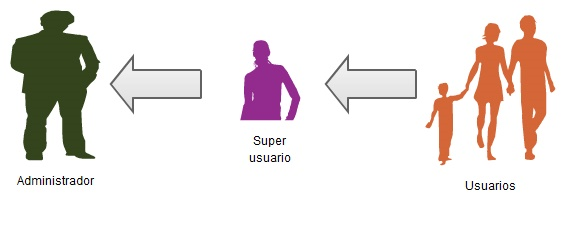
\includegraphics[width=0.7\textwidth]{4.Disenio/Imagenes/Actores}
\end{center}



\section{Casos de uso}
\subsection{Visión general de los casos de uso}
En esta sección se representan las funcionalidades y comportamientos del sistema dependiendo del tipo de usuario que se encuentre en el entorno. Gracias al estudio de los requisitos del sistema, hemos obtenido los casos de uso del sistema de una forma en la que así se agiliza el diseño del sistema y por lo tanto, su posterior implementación.
 
Mostramos a través de las figuras ~\ref{fig:cuSuperusuario} y ~\ref{fig:cuSuperusuario} los diagrama de casos de uso tanto del \textit{Super usuario} como del \textit{Administrador}. Evitamos incluir el diagrama del \textit{Usuario} ya que el \textit{Super usuario} es una extensión de este.

\begin{figure}[h!]
	\centering
	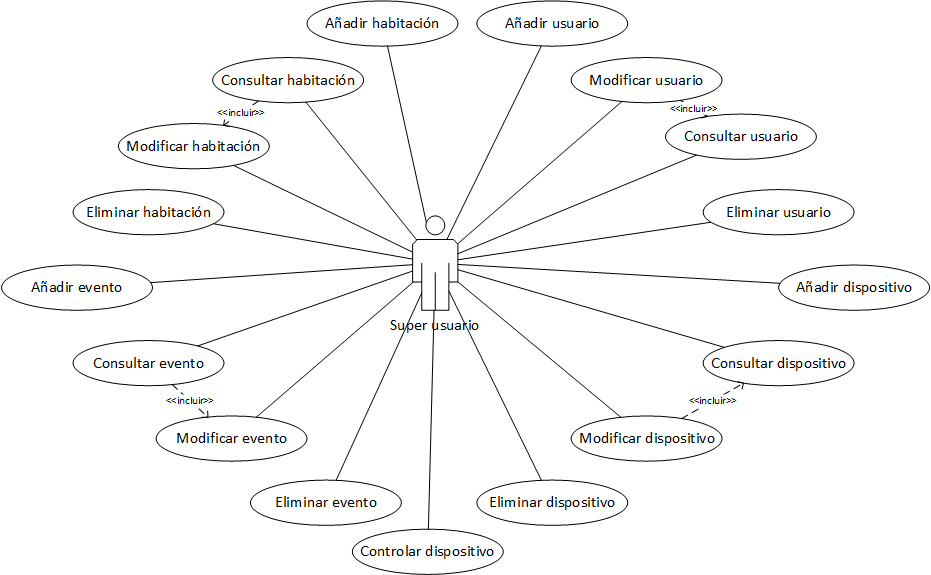
\includegraphics[width=0.7\textwidth]{4.Disenio/Imagenes/CU-Superusuario}
	\caption{Casos de uso del super usuario.}
	\label{fig:cuSuperusuario}
\end{figure}

\begin{figure}[h!]
	\centering
	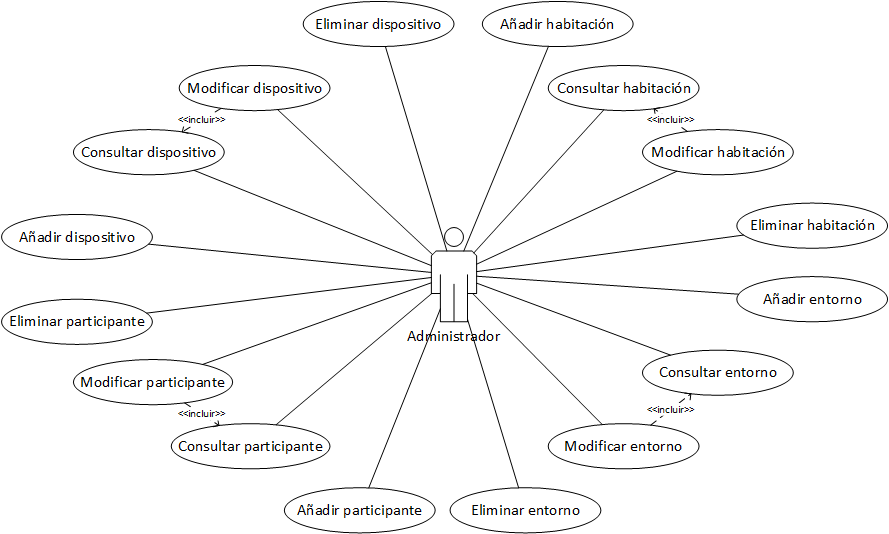
\includegraphics[width=0.7\textwidth]{4.Disenio/Imagenes/CU-Admin}
	\caption{Casos de uso del administrador.}
	\label{fig:cuAdmin}
\end{figure}


\subsection{Casos de uso en detalle}
Debido a la gran cantidad de casos de uso que hemos analizado en el sistema, la información detallada de cada uno de los casos de uso,o comúnmente conocido como \textit{Vista de escenarios}, están localizados en el documento de \textit{Casos de uso}.
\chapter{Vista l\'ogica}
\section{Introducci\'on}
Muestra los componentes principales de dise\~no del sistema y sus relaciones de forma independiente de los detalles tecnicos y de c\'omo la funcionalidad ser\'a implementada. Describiremos esta vista a trav\'es de clases, paquetes, casos de uso y subsistemas.
\section{Principales paquetes de dise\~no}

La aplicaci\'on EHC se descompone en grandes paquetes: [MIRAR ESTOS PUNTOS, NO ME CONVENCEN PARA NADA]
\begin{enumerate}
\item Presentaci\'on: Los usuarios acceder\'an al sistema a trav\'es de diferentes plataformas pero con la misma funcionalidad. Estas plataformas son:
\begin{enumerate}
\item Web: podr\'an acceder a trav\'es de cualquier ordenador con conexi\'on local (si se encuentra en el entorno EHC) o por Internet.
\item M\'ovil: dispondr\'an tanto de una aplicaci\'on para iOS como para Android.
\end{enumerate}
\item Aplicaci\'on: en este paquete englobamos todo aquello a la l\'ogica de la aplicaci\'on. Este paquete engloba:
\begin{enumerate}
\item La propia aplicaci\'on que se encarga de la propia l\'ogica de la aplicaci\'on y de operaciones sencillas.
\item Servidor: se encarga ser el enlace entre el dispositivo m\'ovil o p\'agina web y el entorno EHC.
\end{enumerate}
\item Datos: Base de datos en la nube.
\end{enumerate}

\begin{figure}[h!]
	\centering
	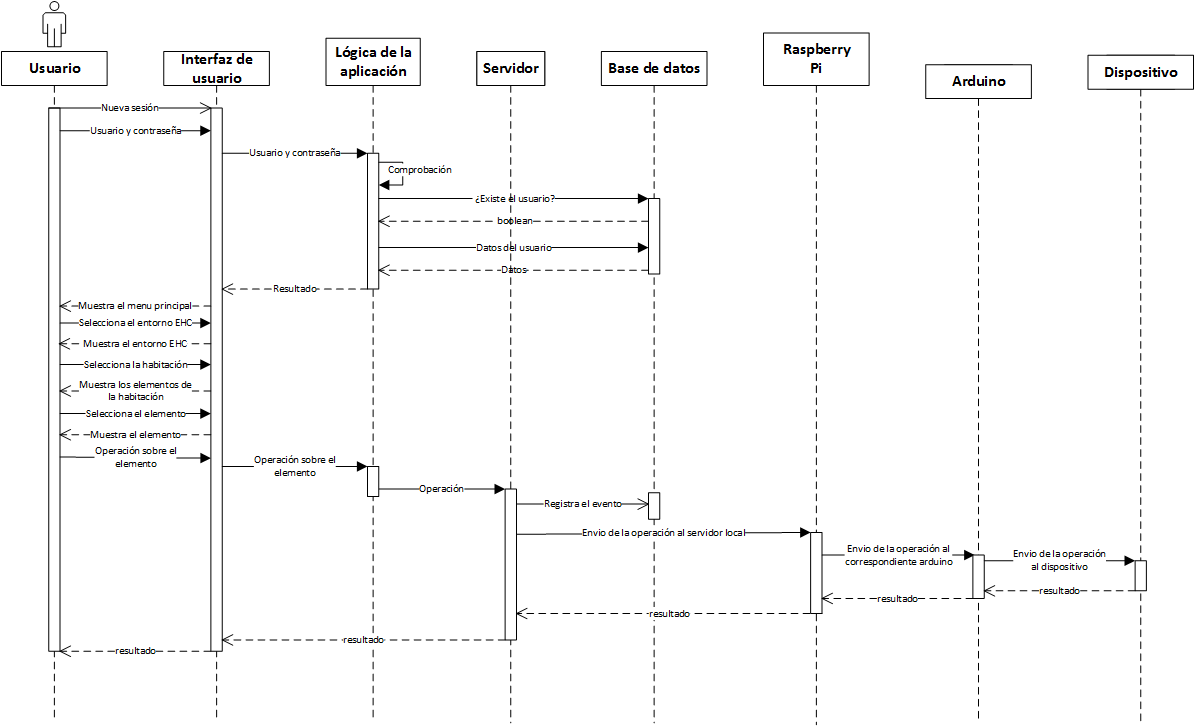
\includegraphics[width=0.9\textwidth]{4.Disenio/Imagenes/DisenioEHC}
	\caption{Diagrama de secuencia de la autentificaci\'on en el sistema y controlar un dispositivo.}
	\label{fig:diagramaSecuencia}
\end{figure}

\begin{figure}
	\centering
	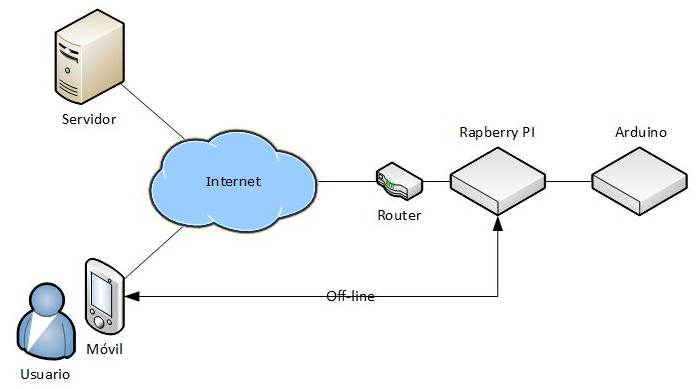
\includegraphics[width=0.8\textwidth]{4.Disenio/Imagenes/arquitectura}
	\caption{Arquitectura del sistema.}
	\label{fig:arquitectura}
\end{figure}


\begin{figure}
	\centering
	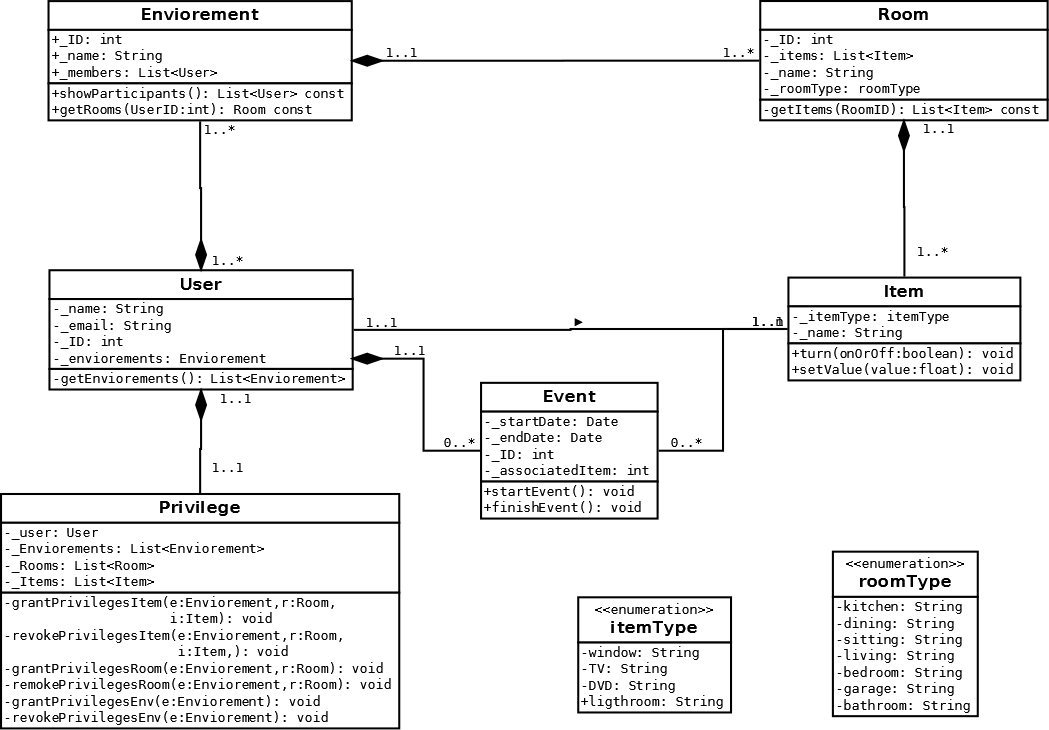
\includegraphics[width=0.8\textwidth]{4.Disenio/Imagenes/diagramaClase}
	\caption{Arquitectura del sistema.}
	\label{fig:diagramaClase}
\end{figure}



(Introducir diagrama de clases, diagrama de comunicacion y diagrama de secuencia)


\chapter{Vista de proceso}
El objetivo es mostrar que hace el sistema en alto nivel y toma en cuenta alguno de los ya citados requisitos no funcionales como es el rendimiento y la disponibilidad. Se describen tareas, sus interacciones y configuraciones, y la asignaci\'on de objetos del dise\~no y clases a las tareas. 
Este tipo de vista es fundamental para sistemas en el que el grado de concurrencia es elevado.
La arquitectura de procesos se describe en varios niveles de abstracci\'on donde cada uno de ellos tienen una funci\'on determinada.

(DIAGRAMA DE ACTIVIDAD)
\chapter{Vista de desarrollo}
Esta vista es fundamental como punto de partida para el equipo de desarrollo para saber como iniciar y organizar el código. El software quedará dividido en varios subsistemas (que a su vez están organizados en capas o jerarquías) que pueden ser desarrollados por uno o varios desarrolladores.

Para poder definir esta vista, previamente se ha tenido que identificar y definir todos los elementos del software.

(Incluir diagrama de paquetes y diagrama de componentes)

\begin{figure}
	\centering
	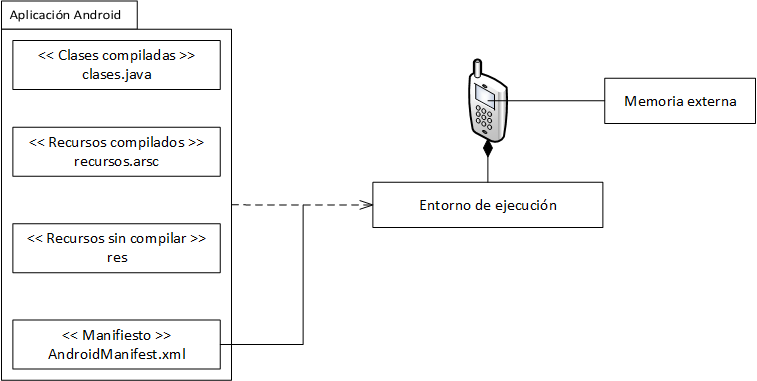
\includegraphics[width=0.65\textwidth]{4.Disenio/Imagenes/AppAndroid}
	\caption{Despliegue de la aplicación Android.}
	\label{fig:appAndroid}
\end{figure}

\chapter{Vista de implementación}

\section{Introducción}
Esta seccion describe la estructura general de la implementaicon del sistema. Muesta la descomposicion del sistema en subsistemas y cuales de estos son los mas importantes. Comprende a grandes rasgos todos aquellos artefactos que se utilizan para ensamblar el sistema y ponerlo en producción, ya listo para su distribución física

La arquitectura del sistema esta distribuida en 3 capas
\begin{enumerate}
\item Presentaci\'on: Esta constituida por todos aquellos componentes visibles para el usuario junto con pequeños submodulos de validacion de datos de entrada y salida. Los usuarios, podrán acceder a esta capa de presentación a través de las siguientes plataformas:
\begin{enumerate}
\item Web: podr\'an acceder a trav\'es de cualquier ordenador con conexi\'on local (si se encuentra en el entorno EHC) o por Internet.
\item M\'ovil: dispondr\'an tanto de una aplicaci\'on para iOS como para Android. A través de esta plataforma también es posible conectarse via local o via Internet.
\end{enumerate}
\item Aplicaci\'on: en esta capa englobamos todo aquello a la l\'ogica de la aplicaci\'on, además de proveer toda la lógica funcional para conectar la capa de presentación con la capa de transferencia de datos . 
\item Datos:   Esta capa consiste en una base de datos MYSQL que provee persistencia de datos. Se sirve de "procedimientos almacenados" que poseen acceso directo a los propipos datos de la base de datos con lo que se consigue fluidez y buena respuesta en la base de datos
    Esta capa se comunica con la capa de Servicio Web para responder a las peticions SQL.
\end{enumerate}


\section{Vista general del sistema}

La arquitectura del sistema está definida en la figura ~\ref{fig:arquitectura}. En dicha figura, podemos destacar los siguientes elementos y características:
\begin{itemize}
\item Dispositivo: el acceso al sistema EHC se puede realizar mediante:
\begin{itemize}
\item Dispositivo móvil: usando las aplicaciones disponibles tanto para iOS como para Android.
\item Ordenador: a través del portal EHC.
\end{itemize}
\item Servidor: será el encargado de enviar las peticiones del usuario a desde el dispositivo origen al entorno EHC a través de Internet. También será el encargado de almacenar toda la información requerida para el sistema.
\item Router: será necesario para poder almacenar la información del entorno EHC y para poder enviar/recibir peticiones a través de Internet.
\item Raspberry PI: funcionará como servidor local del entorno EHC. Será el encargado de gestionar las peticiones recibidas a través de la red local y/o de Internet hacia los dispositivos domotizados del hogar.
\item Arduino: es el subsistema encargado de controlar todos los sensores y actuadores instalados en un dispositivo.
\item Envio de peticiones: como ya se ha mencionado, estas peticiones pueden realizarse a través de Internet o a través de una red local donde estén conectados tanto el terminal origen como el servidor local.
\end{itemize}

\begin{figure}[h!]
	\centering
	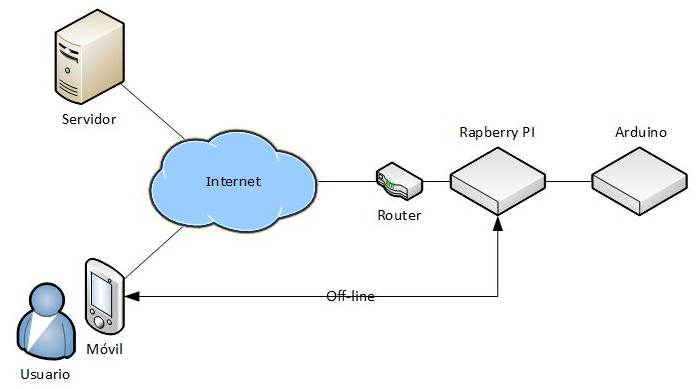
\includegraphics[width=0.8\textwidth]{4.Disenio/Imagenes/arquitectura}
	\caption{Arquitectura del sistema.}
	\label{fig:arquitectura}
\end{figure}


%%%%%%%%%%%%%%%%%%%%%%%%%%%%%%%%%%%%%%%%%%%%%%%%%%%%%%%%%%%%%%%%%%%%%%%%%%%%%%%%%%%

\chapter{Vista de datos}

El sistema atiende al siguiente diagrama relacional:


\begin{figure}[h!]
	\centering
	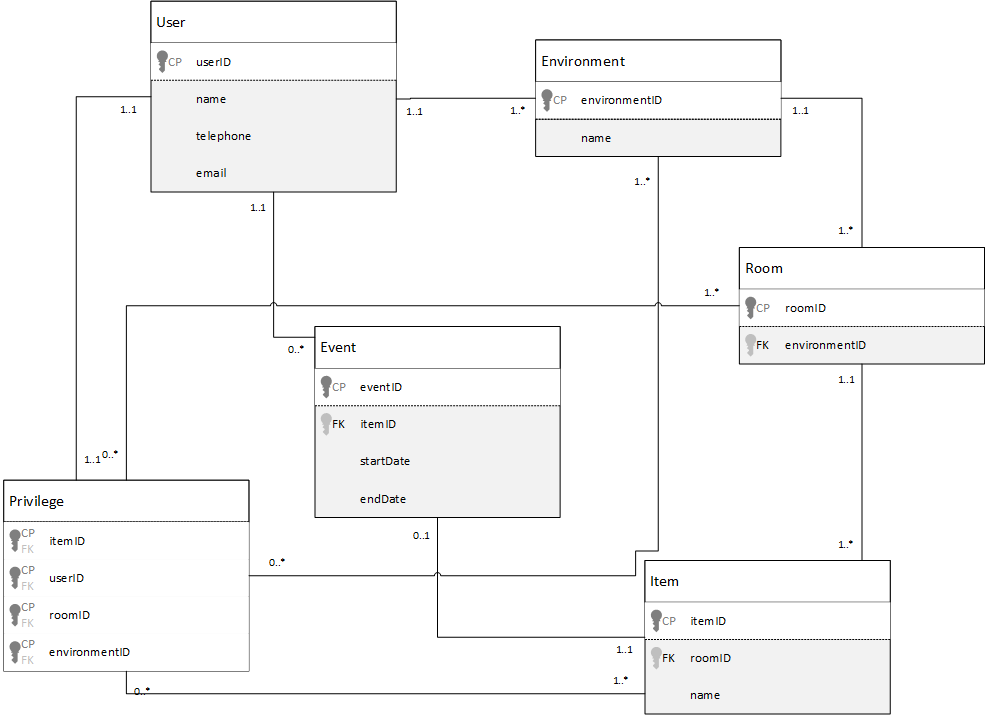
\includegraphics[width=0.8\textwidth]{4.Disenio/Imagenes/ER}
	\caption{Diagrama entidad-relación}
	\label{fig:ER}
\end{figure}








\chapter{Tamaño y rendimiento}

Esta seccion debe contener datos de medidas basadas en aspectos analizables antes de desarrollar el sistema software

Análisis de Puntos de Función

    !Método para cuantificar el tamaño y la complejidad de un sistema de software en términos de las funciones que el sistema entrega al usuario 
    
    •  Método independiente de: 
        "  Lenguaje de programación 
        "  Proceso de desarrollo 
        "  Tecnología 
        "  Capacidad del equipo de desarrollo


[A description of the major dimensioning characteristics of the software that impact the architecture, as well as the target performance constraints.]

Ejemplo de otro proyecto:
    This system currently has mostly listings for the finger lakes region, but the editors are attempting to grow it first to the state level and then eventually to the national level, as such the system had to be designed to allow it to scale up to significantly larger numbers of users and registered organizations.

\chapter{Calidad}
%Puesto que los requisitos de usuario son los mismo que los Funcionales, podriamos omitir las categorias ReqUsuario y ReqSistema y dar por hecho que son todos de sistema (Los de usuario estan expuestos en el documento Vision)


% % % % % % Fin del cuerpo
 %No le gusta la "ñ", asi que las sustituimos por "ni"
    % % Primera página del documento
\begin{titlepage}
    \begin{scriptsize}\noindent Facultad de Informática.\\
        Ingeniería en Informática.\\
        Ingeniería del Software.\\
        Proyecto: Everywhere House Control.
    \end{scriptsize}\\
    \vfill
    \begin{center}
        \begin{Large}
            \textbf{Implementacion y pruebas}
        \end{Large}
    \end{center}
    \vfill
    \begin{flushright}
        \begin{scriptsize}
            \begin{tabular}{lll}
                Creado por & Gutierrez, Hector & Guzman, Fernando  \\
                & Ladrón, Alejandro & Maldonado, Miguel Alexander \\
                & Morales, Álvaro & Ochoa, Victor \\
                & Rey, José Antonio & Saavendra, Luis Antonio  \\
                & Tirado, Colin & Vicente, Victor \\
            \end{tabular}
        \end{scriptsize}
    \end{flushright}
\end{titlepage}
\thispagestyle{empty}
\cleardoublepage
\newpage

% % Tabla de contenidos, etc.
\pagenumbering{Roman}
\tableofcontents
\newpage
\thispagestyle{empty}
\cleardoublepage
\newpage
\pagenumbering{arabic}
\raggedbottom
\interfootnotelinepenalty 10000

%\input{5.Implementacion&Pruebas/...}

% % % % % % Fin del cuerpo

\end{document}

% % % % % % Fin del cuerpo